
A series of combinations are performed corresponding to the Tevatron Run 2 experiments, the LHC experiments, 
all experiments including the result from the LEP combination, and all experiments except one.  For each 
experiment the central value, uncertainty, and $\chi^2$ of the individual measurements is shown for 
the ABMP16, CT14, CT18, MMHT2014, MSHT20, NNPDF31, and NNPDF40 PDF sets.  For the combined result of 
multiple experiments the overall PDF uncertainty is also shown.  The PDF uncertainties for the individual 
experiments are given in Table~\ref{tab:pdfunc}.

%%%% TEVATRON

\subsubsection{Hadron-collider measurements}

Results for the Tevatron Run 2 experiments are listed in Table~\ref{tbl:tevatron_opt2}. The individual 
combinations of the CDF and D0 fit results are satisfactory for all PDF sets, with probabilities ranging
from 12\% to 24\%.  The Tevatron-wide combination has a total uncertainty ranging from 8.9~MeV for ABMP16
to 15.9~MeV for CT18, and a $\chi^2$ probability of 0.5--0.8\%.

As discussed in Section~\ref{sec:corrPDF}, PDF uncertainties are fully correlated between CDF and D0. 
The PDF uncertainty in the combination is therefore close to that obtained for each experiment, and 
ranges from 4~MeV for ABMP16 to 13.5~MeV for CT18. The combined central value ranges from 80408.2~MeV 
for ABMP16 to 80433.4~MeV for NNPDF4.0.  The difference between the NNPDF3.1 and NNPDF4.0 combinations, 
8.4~MeV, is similar to the PDF uncertainty of the NNPDF4.0 set (7.8 MeV).  Similar trends are observed 
for the CDF and D0 measurements separately.  Some variation in the results with PDF set is expected due
to differences in input data sets to the PDFs, and to the differences in the compatibility with Drell-Yan
measurements discussed in Section~\ref{sec:PDFWZ}.  Further understanding of these differences would benefit
future combinations.

\begin{table*}[!tp]
  \centering
  
\begin{tabular*}{\linewidth}{l @{\extracolsep{\fill}}llllllllll}
\hline \hline
   & \multicolumn{2}{c}{CDF (5 d.o.f.)} & & \multicolumn{2}{c}{D0 (4 d.o.f.)} & & \multicolumn{3}{c}{Tevatron Run 2 (1 d.o.f.)} \\
PDF set   & \multicolumn{1}{c}{$m_W$}   & $\chi^2$ & & \multicolumn{1}{c}{$m_W$} & $\chi^2$ & & \multicolumn{1}{c}{$m_W$} & $\sigma_{\scriptsize\textrm{PDF}}$ & $\chi^2$ & p($\chi^2,n$) \\
\hline
   ABMP16 & $80417.3~\pm~9.5$  &  8.8  & & $80355.4 \pm 20.9$ &  6.6   & & $80408.2 \pm  8.9$ &   4.0 &      7.7  & 0.6\% \\
     CT14 & $80432.1 \pm 15.5$ &  7.7  & & $80370.9 \pm 24.9$ &  5.9   & & $80424.0 \pm 15.2$ &  12.6 &      7.2  & 0.7\% \\
     CT18 & $80432.0 \pm 16.1$ &  7.6  & & $80372.0 \pm 25.5$ &  5.9   & & $80424.9 \pm 15.9$ &  13.5 &      7.0  & 0.8\% \\
 MMHT2014 & $80425.7 \pm 11.6$ &  7.0  & & $80364.4 \pm 22.3$ &  5.5   & & $80417.4 \pm 11.2$ &   7.8 &      7.6  & 0.6\% \\
   MSHT20 & $80424.4 \pm 12.2$ &  7.6  & & $80362.3 \pm 22.5$ &  6.1   & & $80415.9 \pm 11.8$ &   8.6 &      7.8  & 0.5\% \\
 NNPDF3.1 & $80433.3 \pm 10.9$ &  7.6  & & $80372.7 \pm 21.9$ &  5.8   & & $80425.0 \pm 10.5$ &   6.8 &      7.4  & 0.7\% \\
 NNPDF4.0 & $80441.8 \pm 11.6$ &  7.2  & & $80381.3 \pm 22.2$ &  5.7   & & $80433.4 \pm 11.2$ &   7.8 &      7.4  & 0.7\% \\
\hline \hline 
\end{tabular*}

  \caption{The CDF and D0 Run 2 $m_W$ and $\chi^2$ values obtained from a combination of the individual
  measurement distributions and decay channels, along with the combined Tevatron Run 2 $m_W$, PDF uncertainty,
  $\chi^2$, and probability of obtaining this $\chi^2$ or larger.  Mass units are in MeV.
}
\label{tbl:tevatron_opt2}
\end{table*}

%%%%% LHC

The LHC results are summarized in Table~\ref{tbl:lhc_opt2}. The $\chi^2$ per degree of freedom of the ATLAS
combination ranges from 29/27 (for NNPDF3.1) to 45/27 (for MSHT20).  The latter corresponds to a probability
of about 2\%.  The larger $\chi^2$ for MSHT20 is consistent with the calculations of Drell-Yan measurements. 
%discussed in Section~\ref{sec:PDFWZ}.
The ATLAS and LHCb measurements are compatible and have a total
uncertainty ranging from 14.2~MeV to 16.6~MeV.

\begin{table*}[!tp]
  \centering
  \begin{tabular*}{\linewidth}{l @{\extracolsep{\fill}}llllllllll}
\hline \hline
           &   \multicolumn{2}{c}{ATLAS (27 d.o.f)} & & \multicolumn{2}{c}{LHCb} & & \multicolumn{3}{c}{LHC (1 d.o.f)} \\
PDF set    & \multicolumn{1}{c}{$m_W$}  & $\chi^2$ & & \multicolumn{1}{c}{$m_W$} & $\chi^2$ & & \multicolumn{1}{c}{$m_W$} & $\sigma_{\scriptsize\textrm{PDF}}$ & $\chi^2$ & p($\chi^2,n$) \\
\hline 
    ABMP16 & $80352.8 \pm 16.1$ & 31 & & $80361.0 \pm 30.4$ & --  & & $80354.6 \pm 14.2$ &    2.9 &    0.1 & 75\% \\
      CT14 & $80363.1 \pm 20.4$ & 30 & & $80354.4 \pm 32.2$ & --  & & $80360.4 \pm 16.4$ &    6.5 &    0.0 & 100\% \\
      CT18 & $80374.5 \pm 20.3$ & 30 & & $80347.3 \pm 32.7$ & --  & & $80366.5 \pm 16.6$ &    6.3 &    0.5 & 48\% \\
  MMHT2014 & $80372.8 \pm 18.6$ & 30 & & $80342.5 \pm 31.3$ & --  & & $80364.4 \pm 15.4$ &    5.1 &    0.6 & 44\% \\
    MSHT20 & $80368.9 \pm 17.9$ & 45 & & $80351.3 \pm 31.0$ & --  & & $80364.3 \pm 15.0$ &    4.5 &    0.2 & 65\% \\
  NNPDF3.1 & $80358.4 \pm 17.6$ & 29 & & $80359.3 \pm 31.1$ & --  & & $80358.6 \pm 15.0$ &    5.0 &    0.0 & 100\% \\
  NNPDF4.0 & $80353.5 \pm 16.6$ & 35 & & $80361.6 \pm 30.6$ & --  & & $80355.4 \pm 14.5$ &    3.8 &    0.1 & 75\% \\
\hline \hline
\end{tabular*}

  \caption{The ATLAS and LHCb $m_W$ values obtained from a combination of the individual measurement distributions
  and decay channels, along with the combined LHC $m_W$, PDF uncertainty, and $\chi^2$, and probability of obtaining
  this $\chi^2$ or larger.  The $\chi^2$ 
  of the combination of fit distributions and decay channels is shown for ATLAS; no $\chi^2$ is shown for LHCb as the
  measurement is performed using one distribution in one channel.  Mass units are in MeV.
  }
  \label{tbl:lhc_opt2}
\end{table*}

The individual experimental results are shown in Figure~\ref{fig:sumexpt} for all considered PDF sets.
The combination of ATLAS and LHCb measurements benefits from anti-correlated PDF uncertainties~\cite{Bozzi:2015zja}. 
Therefore the combined PDF uncertainties and the variation of the combined central values are smaller than for the 
individual experiments. The ATLAS $m_W$ value ranges from 80352.8~MeV for ABMP16 to 80374.5~MeV for CT18. This range
is comparable to that of the Tevatron experiments. A similar spread but opposite trends are observed for LHCb, and
the spread of $m_W$ values is reduced from $\approx 20$~MeV to 14.1~MeV in the combination. The PDF uncertainties
range from 4.0~MeV to 11.4~MeV for ATLAS and 3.0 to 12.2~MeV for LHCb, but are reduced to 2.9--6.5~MeV for
the combined result.  

\begin{figure}[!tp]
  \centering
  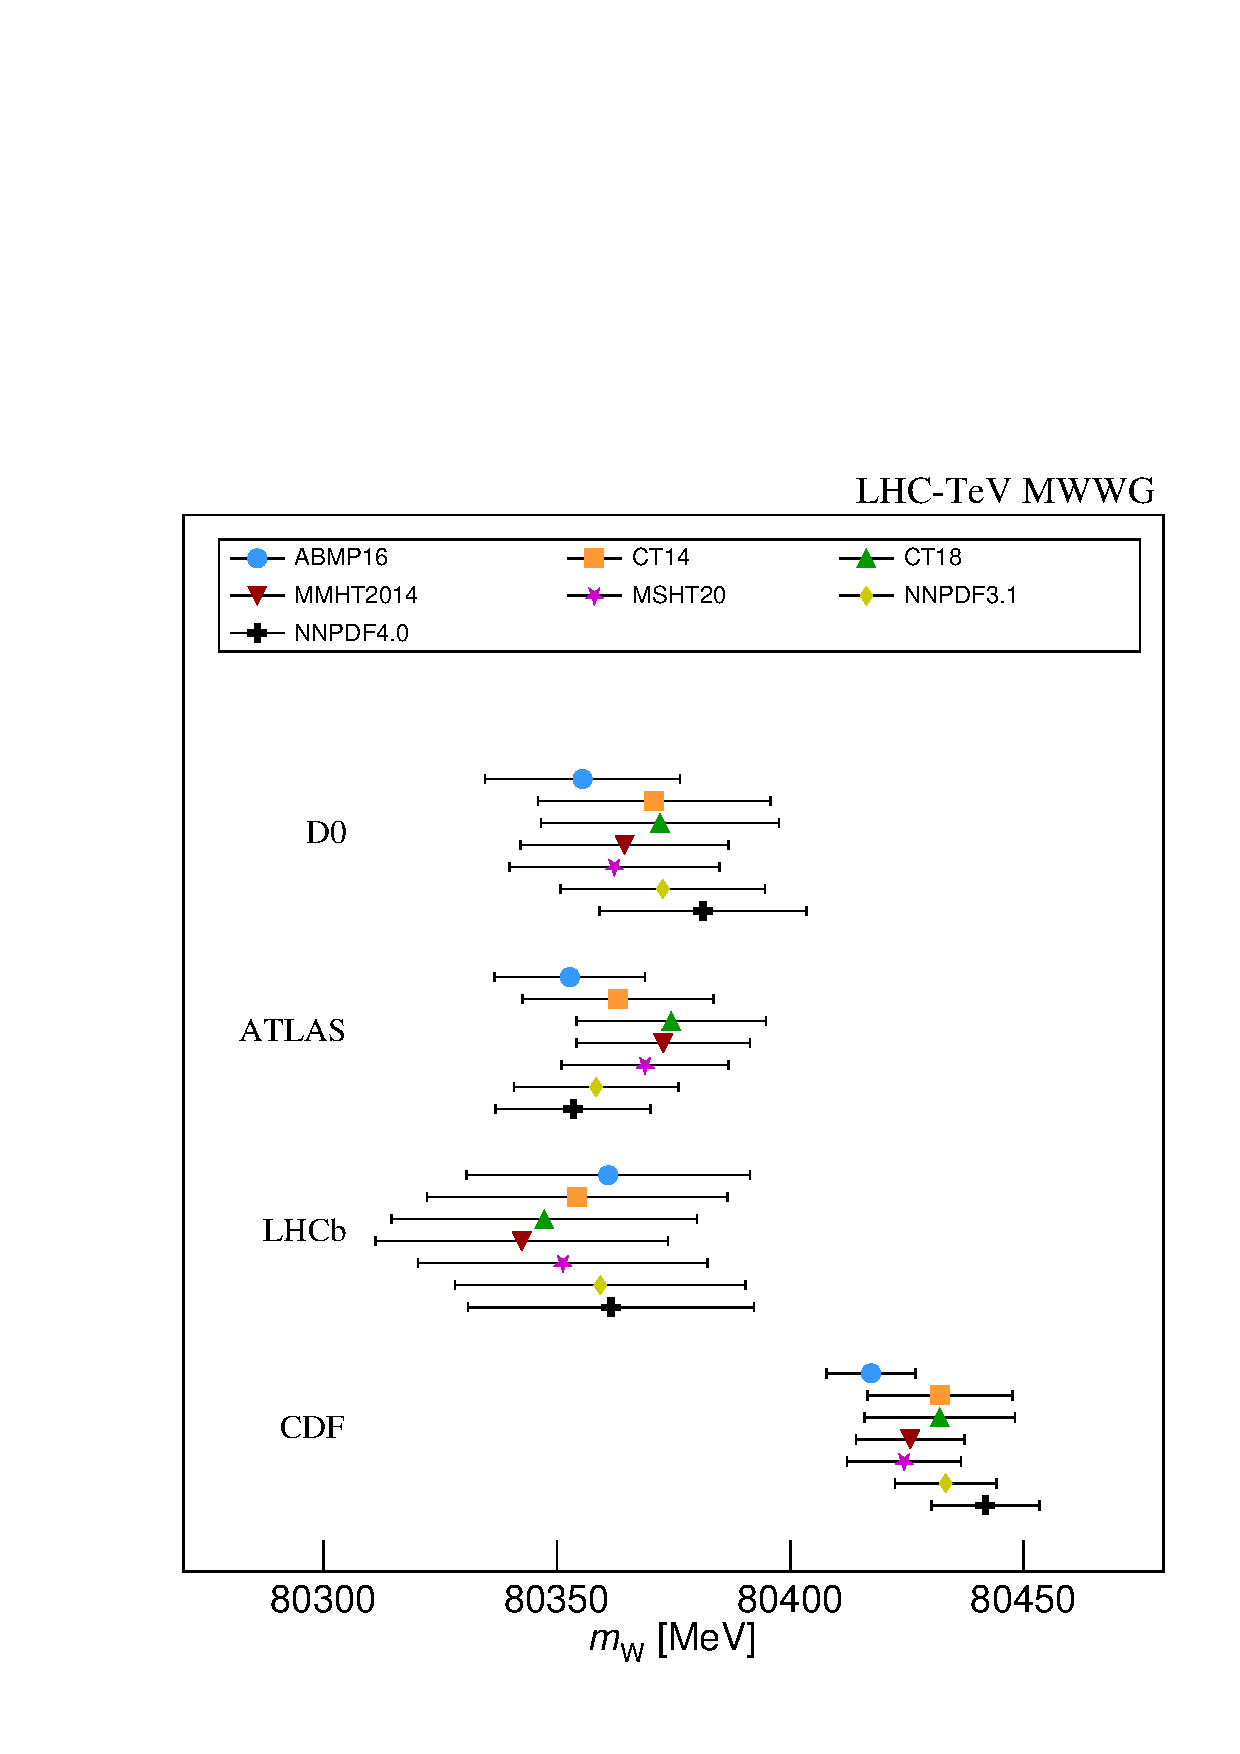
\includegraphics[width=0.95\columnwidth]{summary_plot_experiments.pdf}
  \caption{The D0, ATLAS, LHCb, and CDF $m_W$ values and uncertainties using the ABMP16, CT14, CT18, MMHT2014,
  MSHT20, NNPDF3.1, and NNPDF4.0 PDF sets. 
}
\label{fig:sumexpt}
\end{figure}


%%%% ALL
\subsubsection{All measurements}

Tables~\ref{tbl:all1_opt2}--\ref{tbl:all3_opt2} provide the results for various combinations including
LEP, whose uncertainties are treated as uncorrelated with the others.  A combination of all measurements
yields a total uncertainty ranging between 7.5 and 11.5~MeV, though the $\chi^2$ probabilities are low,
ranging from $8 \times 10^{-6}$ to $5\times 10^{-3}$.  The low probabilities
reflect the discrepancy between the CDF measurement and the other measurements. The combined value of
$m_W$ for the CT18 PDF set, which gives the largest compatibility with the broader Drell-Yan measurements,
is $m_W = 80394.6 \pm 11.5$~MeV with a probability of 0.5\%.  The relative weights of the CDF, ATLAS, LHCb,
LEP, and D0 measurements are 41\%, 28\%, 13\%, 12\%, and 5\%, respectively.  Weights for other PDF sets are
given in the Appendix.  The largest difference in $m_W$ between PDF sets is 10.4 MeV.

  \begin{table}[!tp]
  \centering
\begin{tabular}{lllll}
\hline \hline
                                     \multicolumn{5}{c}{All experiments (4 d.o.f.)} \\
PDF set                      & \multicolumn{1}{c}{$m_W$} & $\sigma_{\scriptsize\textrm{PDF}}$ & $\chi^2$ & p($\chi^2,n$) \\
\hline
                             ABMP16 & $80392.7 \pm  7.5$ &   3.2 &    29  & 0.0008\% \\
                               CT14 & $80393.0 \pm 10.9$ &   7.1 &    16  & 0.3\% \\
                               CT18 & $80394.6 \pm 11.5$ &   7.7 &    15  & 0.5\% \\
                           MMHT2014 & $80398.0 \pm  9.2$ &   5.8 &    17  & 0.2\% \\
                             MSHT20 & $80395.1 \pm  9.3$ &   5.8 &    16  & 0.3\% \\
                           NNPDF3.1 & $80403.0 \pm  8.7$ &   5.3 &    23   & 0.1\% \\
                           NNPDF4.0 & $80403.1 \pm  8.9$ &   5.3 &    28   & 0.001\% \\
\hline \hline
\end{tabular}
\caption{Combination of $m_W$ measurements from the individual experiments.
  Shown for each PDF are the PDF uncertainty, $\chi^2$, and probability of
  obtaining this $\chi^2$ or larger.  Mass units are in MeV.
  \label{tbl:all1_opt2}}
\end{table}


\begin{table}[!tp]
  \centering
\begin{tabular}{lllll}
\hline \hline

                                     \multicolumn{5}{c}{All except LEP (3 d.o.f.)} \\
PDF set                      & \multicolumn{1}{c}{$m_W$} & $\sigma_{\scriptsize\textrm{PDF}}$ & $\chi^2$ & p($\chi^2,n$) \\
\hline
                             ABMP16 & $80393.6 \pm  7.8$ &     3.4 &     19   & 0.03\% \\
                               CT14 & $80395.1 \pm 11.6$ &     8.0 &     16   & 0.1\% \\
                               CT18 & $80397.1 \pm 12.3$ &     8.8 &     15   & 0.2\% \\
                           MMHT2014 & $80399.9 \pm  9.6$ &     6.2 &     17   & 0.7\% \\
                             MSHT20 & $80396.8 \pm  9.7$ &     6.3 &     16   & 0.1\% \\
                           NNPDF3.1 & $80405.0 \pm  9.0$ &     5.6 &     22   & 0.007\% \\
                           NNPDF4.0 & $80405.3 \pm  9.2$ &     5.7 &     27   & 0.0006\% \\
\hline \hline
\end{tabular}
\caption{Combination of all $m_W$ measurements except the LEP average.  Shown for each PDF are the 
  PDF uncertainty, $\chi^2$, and probability of
  obtaining this $\chi^2$ or larger.  Mass units are in MeV.
  \label{tbl:all2_opt2}
}
\end{table}


  
\begin{table}[!tp]
  \centering
\begin{tabular}{lllll}
\hline \hline 
                                       \multicolumn{5}{c}{All except CDF (3 d.o.f.)} \\
PDF set                      & \multicolumn{1}{c}{$m_W$} & $\sigma_{\scriptsize\textrm{PDF}}$ & $\chi^2$ & p($\chi^2,n$) \\
\hline
                             ABMP16 & $80357.3 \pm 11.2$ &  2.6 &  0.4 & 94\% \\
                               CT14 & $80365.4 \pm 12.9$ &  5.8 &  0.3 & 96\% \\
                               CT18 & $80369.2 \pm 13.3$ &  6.2 &  0.5 & 92\% \\
                           MMHT2014 & $80365.8 \pm 12.1$ &  4.7 &  0.8 & 85\% \\
                             MSHT20 & $80365.1 \pm 12.0$ &  4.4 &  0.4 & 94\% \\
                           NNPDF3.1 & $80364.7 \pm 11.9$ &  4.5 &  0.4 & 94\% \\
                           NNPDF4.0 & $80364.5 \pm 11.6$ &  3.9 &  1.2 & 75\% \\
\hline \hline
\end{tabular}
\caption{Combination of $m_W$ measurements from all individual experiments except CDF.
  Shown for each PDF are the PDF uncertainty, $\chi^2$, and probability of
  obtaining this $\chi^2$ or larger.  Mass units are in MeV.
  \label{tbl:all3_opt2}}
\end{table}



\begin{table}[!tp]
  \centering
\begin{tabular}{lllll}
\hline \hline 
                                    \multicolumn{5}{c}{All except D0 (3 d.o.f.)} \\
PDF set                      & \multicolumn{1}{c}{$m_W$} & $\sigma_{\scriptsize\textrm{PDF}}$ & $\chi^2$ & p($\chi^2,n$)\\
\hline
                             ABMP16 & $80397.2 \pm  7.8$ &  3.1 &    15 & 0.2\% \\
                               CT14 & $80395.9 \pm 11.0$ &  7.0 &    11 & 1.2\% \\
                               CT18 & $80397.1 \pm 11.6$ &  7.6 &    10 & 1.9\% \\
                           MMHT2014 & $80401.9 \pm  9.4$ &  5.6 &    13 & 0.5\% \\
                             MSHT20 & $80399.0 \pm  9.5$ &  5.7 &    12 & 0.7\% \\
                           NNPDF3.1 & $80406.6 \pm  8.9$ &  5.1 &    19 & 0.03\% \\
                           NNPDF4.0 & $80406.4 \pm  9.0$ &  5.1 &    25 & 0.002\% \\
\hline \hline
\end{tabular}
\caption{Combination of $m_W$ measurements from all individual experiments except D0.
  Shown for each PDF are the PDF uncertainty, $\chi^2$, and probability of
  obtaining this $\chi^2$ or larger.  Mass units are in MeV.
  \label{tbl:all4_opt2}}
\end{table}


  

\begin{table}[!tp]
  \centering
  \begin{tabular}{lllll}
\hline \hline
                              \multicolumn{5}{c}{All except ATLAS (3 d.o.f.)} \\
PDF set                      & \multicolumn{1}{c}{$m_W$} & $\sigma_{\scriptsize\textrm{PDF}}$ & $\chi^2$ & p($\chi^2,n$)\\
\hline 
                             ABMP16 & $80402.8 \pm  8.3$ &  3.5 & 11 & 1.2\% \\
                               CT14 & $80406.5 \pm 12.8$ &  9.1 & 12 & 0.7\% \\
                               CT18 & $80405.0 \pm 13.2$ &  9.6 & 13 & 0.5\% \\
                           MMHT2014 & $80405.8 \pm 10.0$ &  6.3 & 14 & 0.3\% \\
                             MSHT20 & $80404.2 \pm 10.3$ &  6.6 & 12 & 0.7\%  \\
                           NNPDF3.1 & $80414.7 \pm  9.5$ &  5.6 & 13 & 0.5\%  \\
                           NNPDF4.0 & $80420.2 \pm 10.0$ &  6.2 & 14 & 0.3\% \\
                            \hline \hline 
%\bottomrule
\end{tabular}
  \caption{Combination of $m_W$ measurements from the individual experiments except for ATLAS.
      Shown for each PDF are the PDF uncertainty, $\chi^2$, and probability of
  obtaining this $\chi^2$ or larger.  Mass units are in MeV.
    \label{tbl:all5_opt2}}
\end{table}


\begin{table}[!tp]
  \centering  
\begin{tabular}{lllll}
\hline \hline
                            \multicolumn{5}{c}{All except LHCb (3 d.o.f.)} \\
PDF set                   & \multicolumn{1}{c}{$m_W$} & $\sigma_{\scriptsize\textrm{PDF}}$ & $\chi^2$ & p($\chi^2,n$) \\
\hline 
                          ABMP16 & $80394.8 \pm  7.7$ & 3.4 &   18 & 0.04\%  \\
                            CT14 & $80399.8 \pm 11.7$ & 8.4 &   14 & 0.3\% \\
                            CT18 & $80402.6 \pm 12.4$ & 9.0 &   12 & 0.7\% \\
                        MMHT2014 & $80404.4 \pm  9.7$ & 6.5 &   13 & 0.5\% \\
                          MSHT20 & $80400.7 \pm 10.0$ & 6.8 &   14 & 0.3\% \\
                        NNPDF3.1 & $80407.4 \pm  9.1$ & 5.8 &   20 & 0.02\% \\
                        NNPDF4.0 & $80407.3 \pm  9.3$ & 5.9 &   26 & 0.001\% \\
\hline \hline 
%\bottomrule
\end{tabular}
  \caption{Combination of $m_W$ measurements from the individual experiments except for LHCb.
          Shown for each PDF are the PDF uncertainty, $\chi^2$, and probability of
  obtaining this $\chi^2$ or larger.  Mass units are in MeV.
    \label{tbl:all6_opt2}}
\end{table}



A possible procedure for combining measurements with low compatibility is to scale all uncertainties by the
square root of the ratio of the $\chi^2$ to the number of degrees of freedom.
This procedure effectively assumes a common underestimated uncertainty, which is an unlikely scenario for
these measurements.  The PDF uncertainty is only partially correlated, and the uncertainty from the CT18 set
is the most conservative.  Other measurement uncertainties are smaller or are statistically constrained and
therefore uncorrelated.  Further measurements or studies are required to obtain more consistent results.

To evaluate the significance of differences between individual measurements and the others, separate
combinations are performed excluding, in turn, each individual result from the average.
Removing LEP, D0, or LHCb from the combination increases the uncertainty by up to 0.9~MeV and affects
the central value by up to 8~MeV.
When removing ATLAS the
$\chi^2$ probability ranges from 0.3\% to 1.2\%, and the uncertainty ranges from 8.3~to 13.2~MeV.
The
combinations with CDF excluded have good compatibility and the total uncertainty increases to 11.2--13.3~MeV,
or 2--4~MeV more than the full combination.  The variation of this combination with PDF set is 11.9 MeV, with 
the value for the ABMP16 PDF set considerably lower than the others (the variation is 4.5 MeV without this set).
The combination of all measurements except CDF is $m_W=80369.2 \pm 13.3$~MeV for the CT18 PDF set, with a
91\% probability of consistency.  The relative weights for the ATLAS, D0, LHCb, and LEP measurements are 42\%,
23\%, 18\%, and 16\%, respectively.
 
The partial combinations are also used to evaluate the difference between each experimental result and the
combination of the others. Considering all PDF sets, the LEP result is compatible with the average of the
others to better than one standard deviation. The compatibility of D0 or LHCb with the rest ranges from
1--1.8 standard deviations. The ATLAS result differs from the others by 1.6--3.6 standard deviations,
where the largest difference is obtained with the NNPDF4.0 PDF set. Finally, the CDF measurement differs
from the others by 3.6--5.2 standard deviations, depending on the choice of the PDF set. The smallest 
significance corresponds to the CT18 set and the largest significance corresponds to the NNPDF4.0 set.
 
The $m_W$ combinations from LEP, the Tevatron, the LHC, and all experiments are presented in Figure~\ref{fig:sumcomb}
for all PDF sets, along with the corresponding $\chi^2$ probabilities. The same information is also shown
for the combinations removing one experimental result at a time.

\begin{figure*}[p]
  \centering
  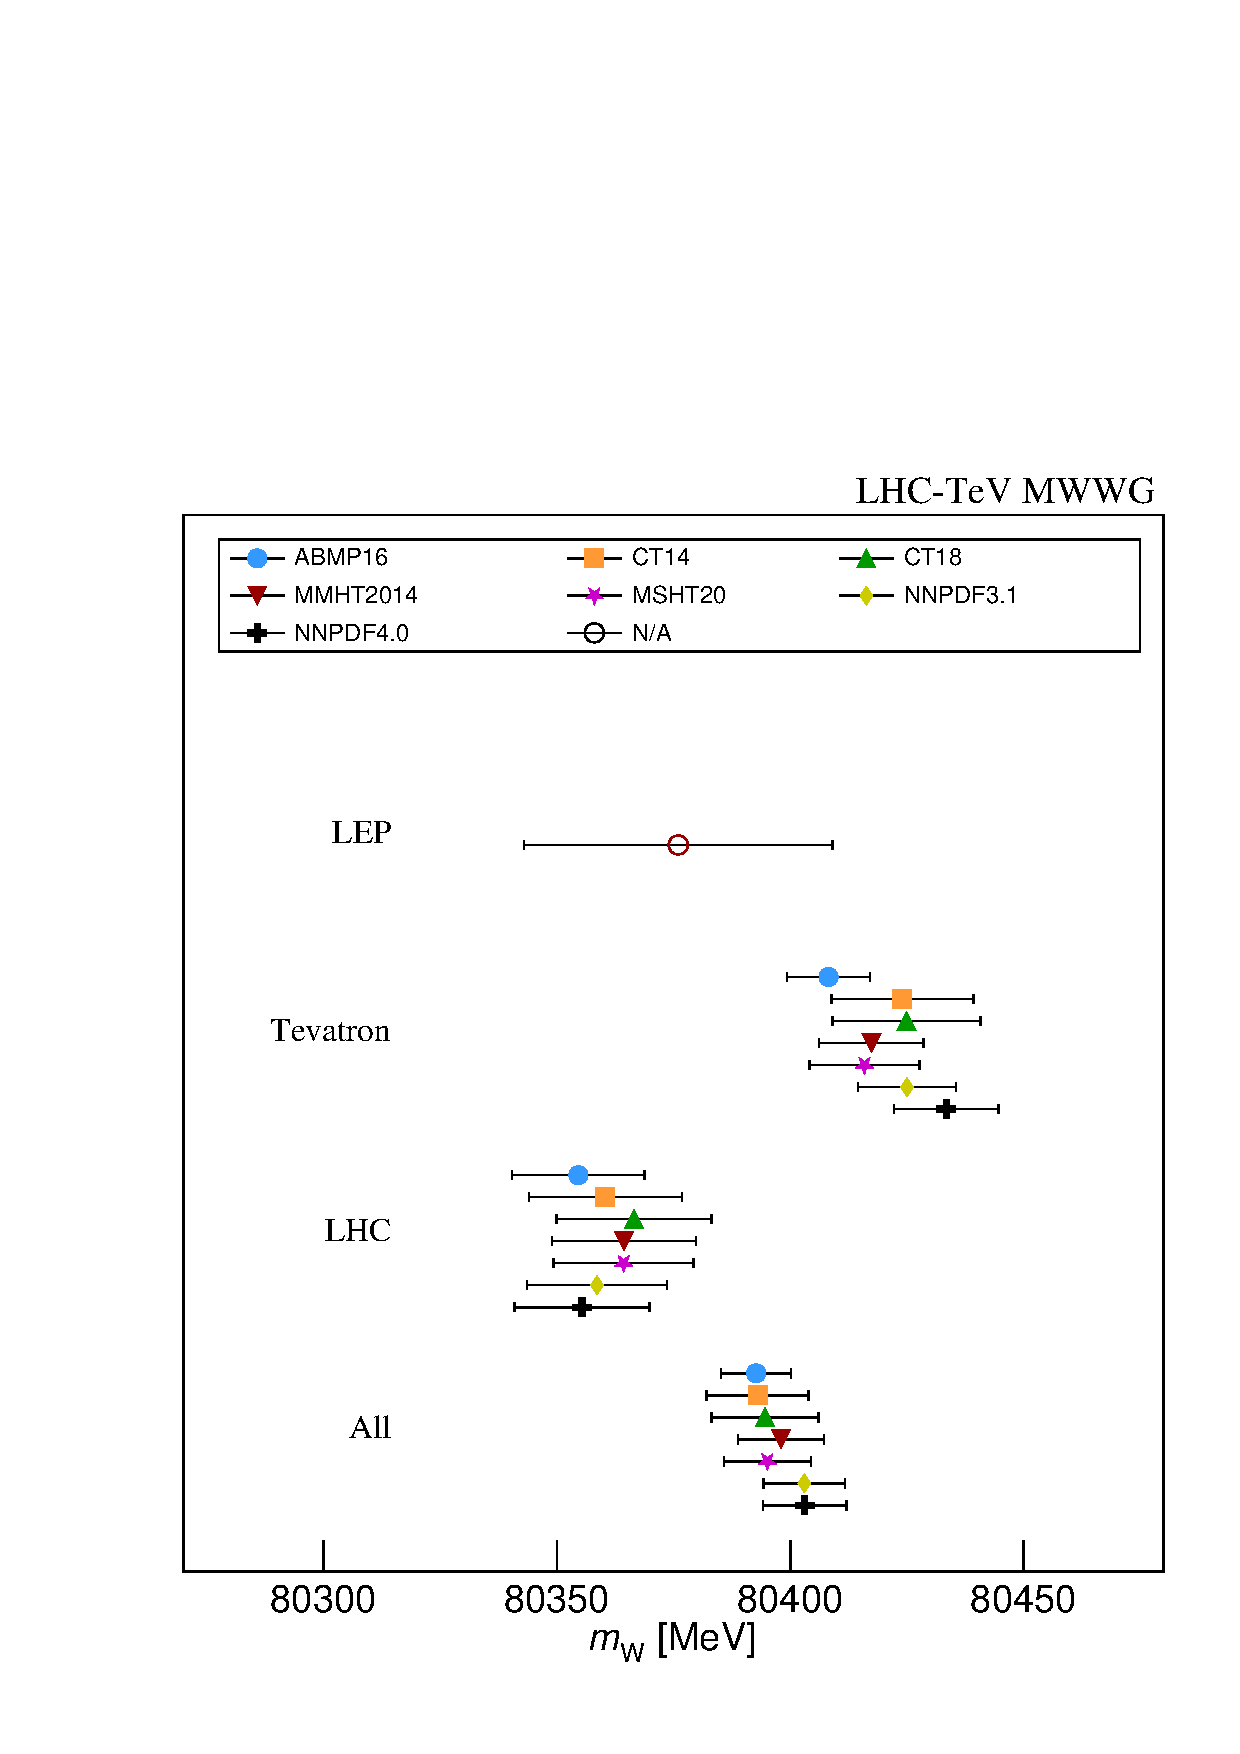
\includegraphics[width=0.95\columnwidth]{summary_plot_subcombinations.pdf}
  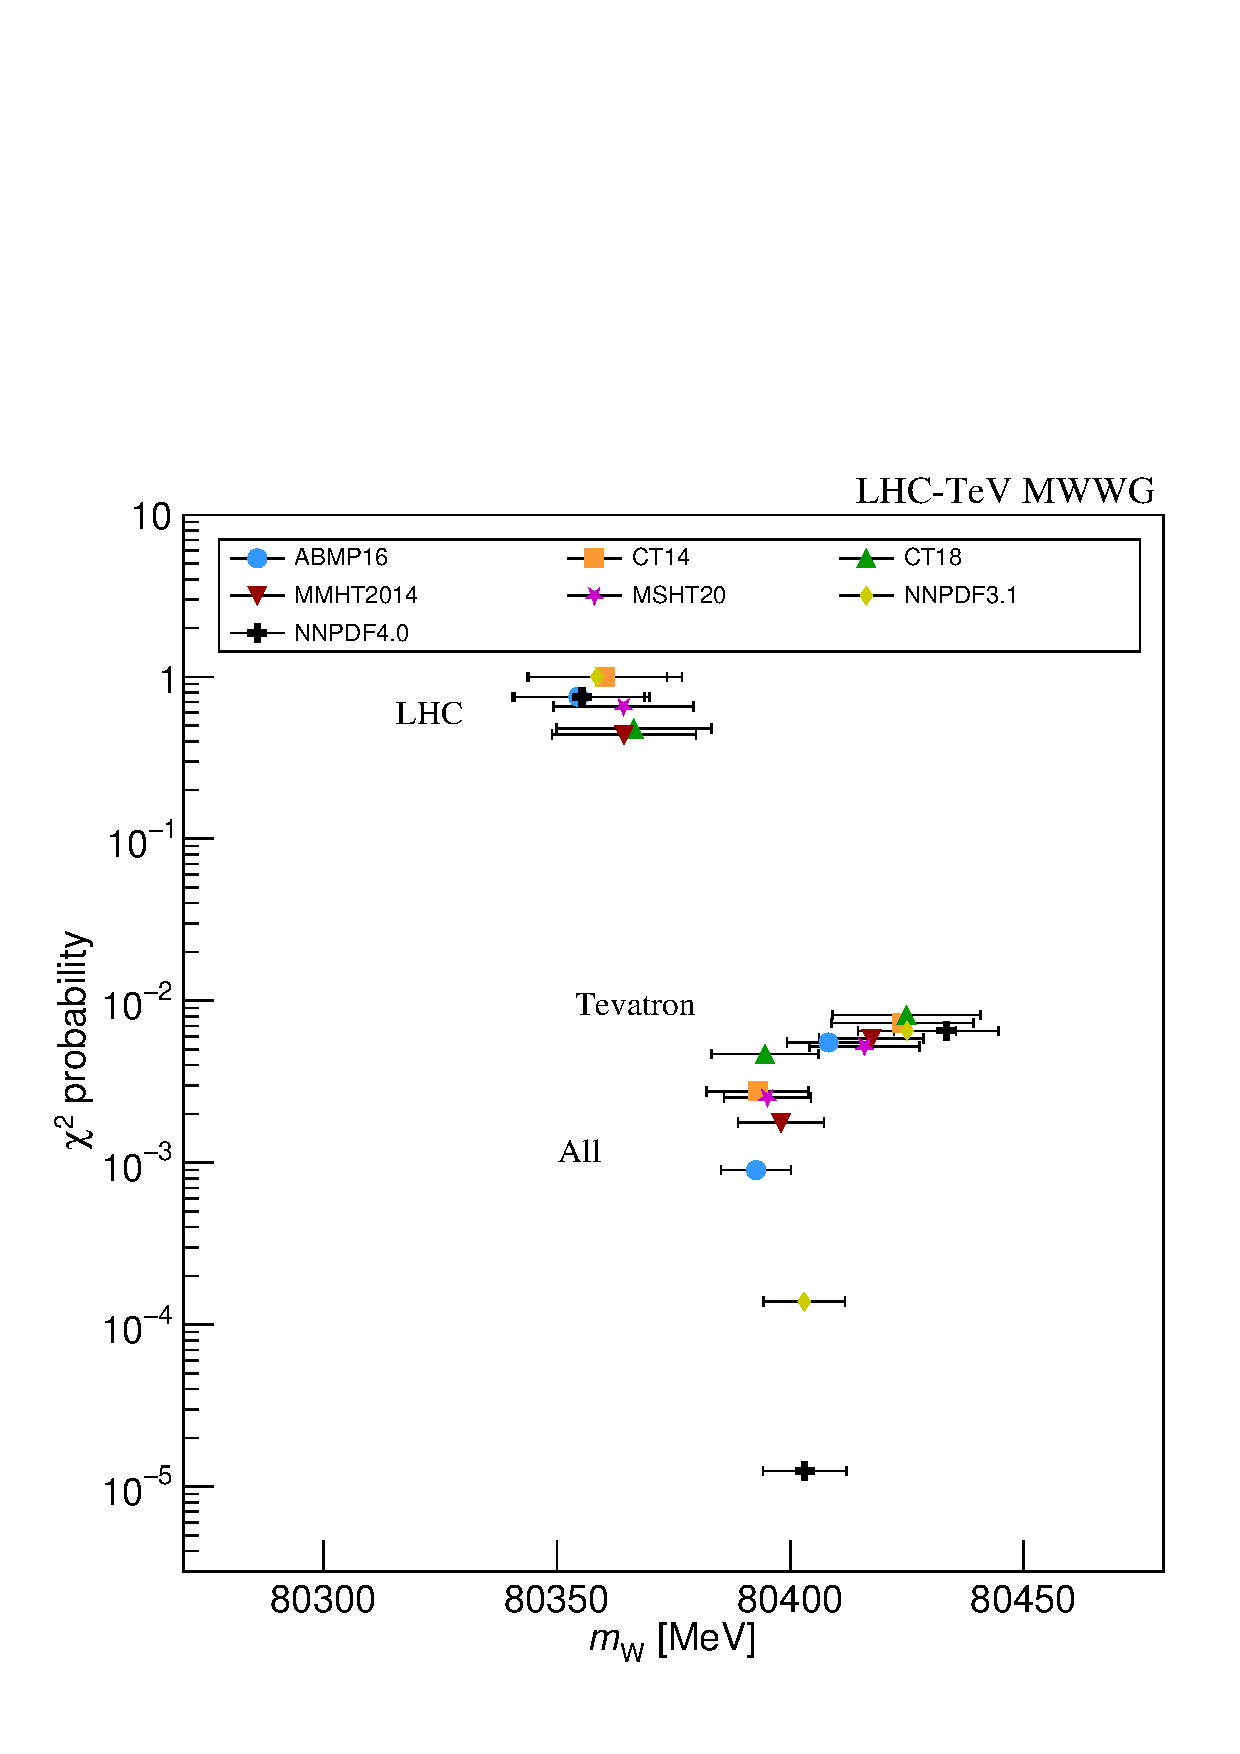
\includegraphics[width=0.95\columnwidth]{summary_plot_2d_subcombinations.pdf}
  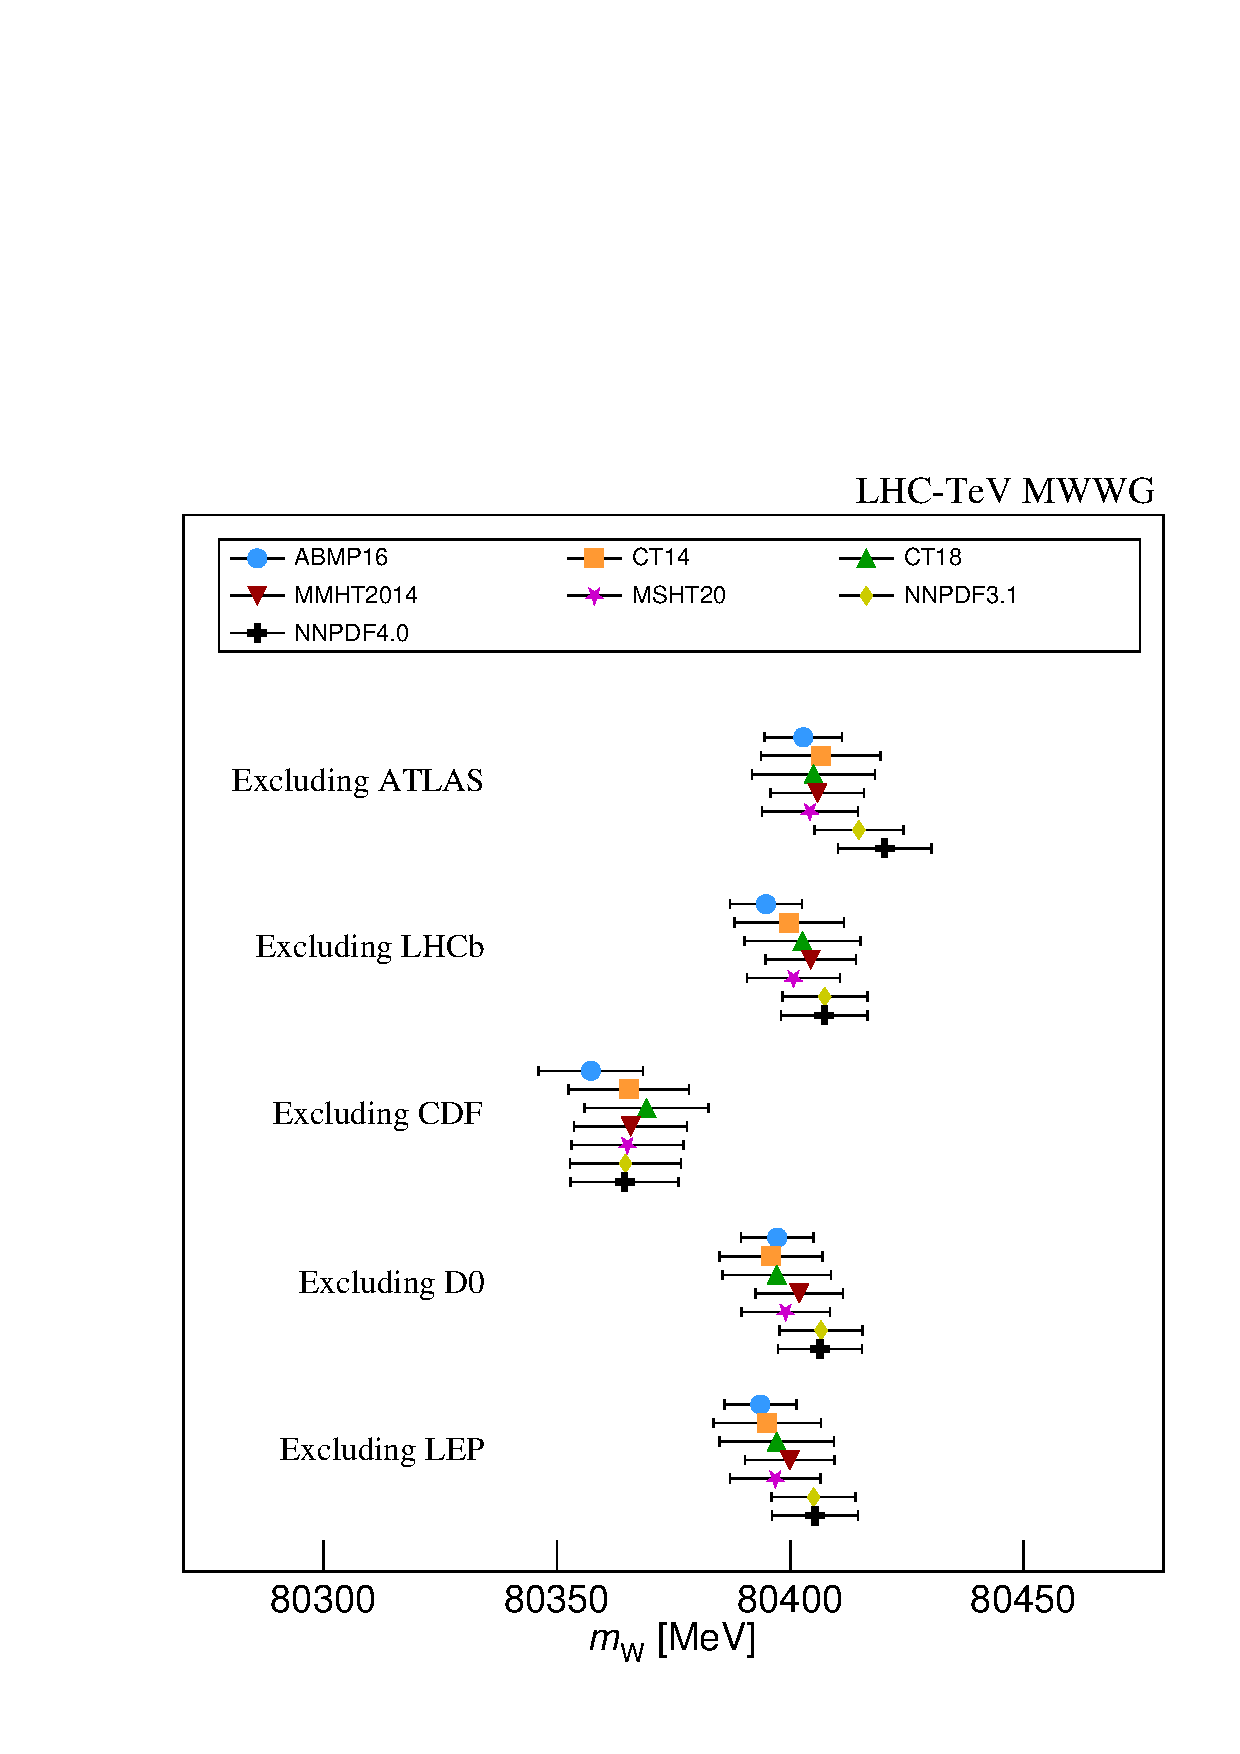
\includegraphics[width=0.95\columnwidth]{summary_plot_exceptions.pdf}
  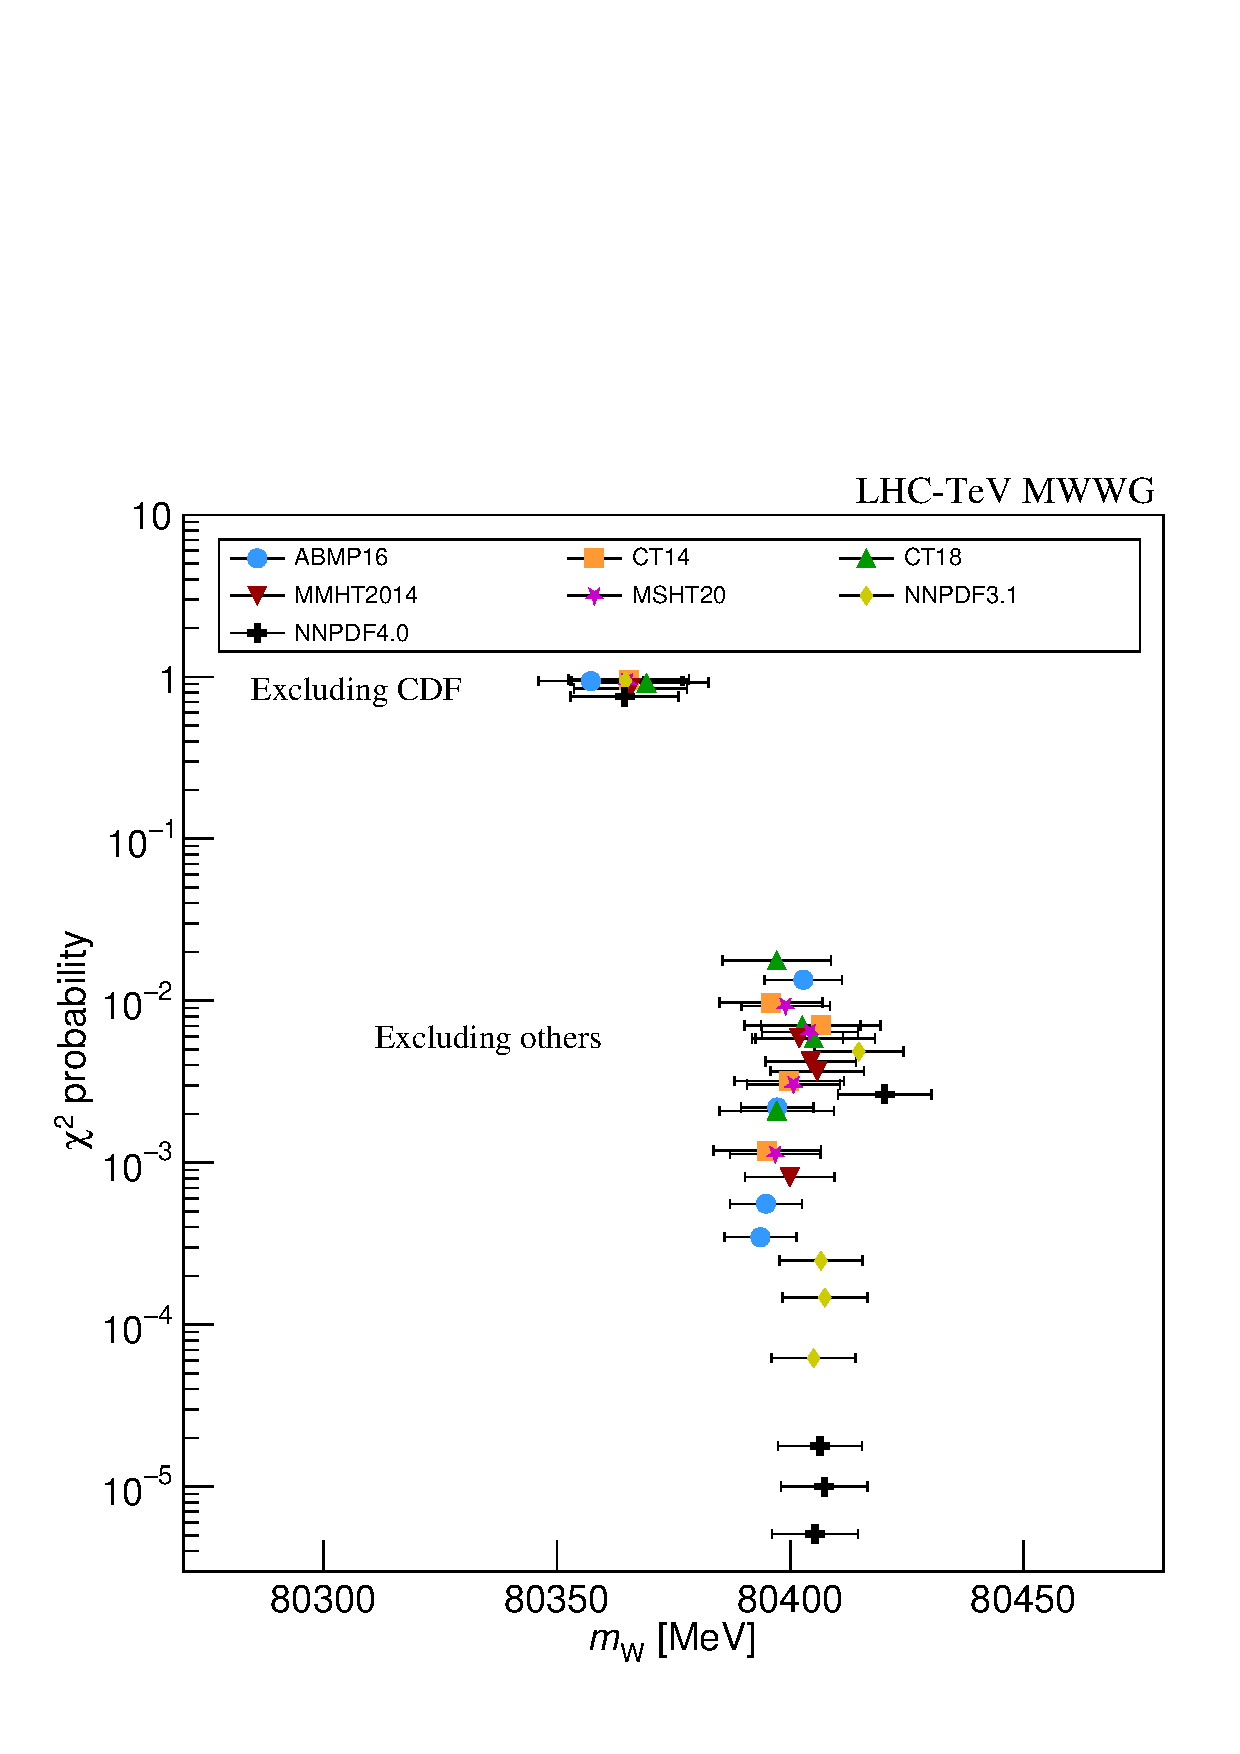
\includegraphics[width=0.95\columnwidth]{summary_plot_2d_exceptions.pdf}
  \caption{Top left: The combined $m_W$ values and uncertainties from LEP, the Tevatron, LHC, and all experiments,
  using the ABMP16, CT14, CT18, MMHT2014, MMHT20, NNPDF3.1, and NNPDF4.0 PDF sets.  Right: The corresponding
  probability of consistency determined using the $\chi^2$ per degrees of freedom.
 Bottom left: The combined $m_W$ values and uncertainties for all experiments except one using the ABMP16,
  CT14, CT18, MMHT2014, MMHT20, NNPDF3.1, and NNPDF4.0 PDF sets.  Right: The corresponding probability of
  consistency determined using the $\chi^2$ per degrees of freedom.
}
  \label{fig:sumcomb}
\end{figure*}

